\section{TINJAUAN PUSTAKA}
\label{sec:tinjauanpustaka}

% Ubah bagian-bagian berikut dengan isi dari tinjauan pustaka

% Demi mendukung penelitian ini, \lipsum[1][1-5]

% \section{Roket Luar Angkasa}
% \label{sec:roketluarangkasa}

% % Contoh input gambar
% \begin{figure}[ht]
%   \centering

%   % Ubah dengan nama file gambar dan ukuran yang akan digunakan
%   \includegraphics[scale=0.35]{gambar/roketluarangkasa.jpg}

%   % Ubah dengan keterangan gambar yang diinginkan
%   \caption{Peluncuran roket luar angkasa \emph{Discovery} \citep{roketluarangkasa}.}
%   \label{fig:roketluarangkasa}
% \end{figure}

% Roket luar angkasa merupakan \lipsum[1]

% \emph{Discovery}, Gambar \ref{fig:roketluarangkasa}, merupakan \lipsum[2]

% \subsection{Deep Learning}
% \label{sec:deeplearning}

% Deep Learning sejatinya bagian machine learning yang dimana algoritma nya terinspirasi dari cara kerja jaringan neuron seperti 
% halnya jaringan neuron pada otak manusia. Pada deep learning, syaraf atau neuron merupakan perwakilan dari satu fungsi yang 
% menyimpan suatu nilai atau value yang dimana neuron - neuron ini berada dalam layer - layer yang dimana antar layer memiliki 
% hubungan tertentu. Deep Learning digunakan karena kemampuanya untuk menemukan relasi yang tidak ditemukan antara input dan output. \cite{Goodfellow-et-al-2016}

% Deep Learning adalah bagian dari machine learning yang dimana juga merupakan bagian dari artificial intelligence yang dimana memiliki metode
% yang lebih tradisional untuk untuk melakukan aksi berdasarkan data. Deep learning adalah teknik machin learning yang dimana mempelajari
% fitur dan tugas langsung dari data dengan cara menyalurkan input melewati neural network yangn mempunyai hidden layer.



% \emph{Discovery}, Gambar \ref{fig:roketluarangkasa}, merupakan \lipsum[2]


\subsection{Helm Keselamatan Kerja}
\label{subsec:helmkeselamatankerja}

\begin{figure}[ht]
    \centering
    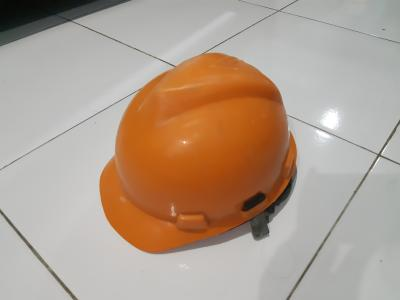
\includegraphics[scale=0.7]{gambar/safety_helmet.jpg}
    \caption{Helm Keselamatan Kerja}
    \label{fig:helmkeselamatankerja}  
  \end{figure}

Helm Keselamatan Kerja seperti helm atau pelindung kepala pada umumnya memiliki kemampuan untuk 
melindungi kepala pengguna. Menurut surat dari Menteri Tenaga Kerja dan Trasmihrasi nomor PER. PER. 08/MENVIII/2010, 
jenis – jenis alat perlindungan diri salah satunya yaitu Alat Pelindung Kepala yang dimana contoh bentuk
nya yaitu helm keselamatan kerja atau safety helmet diantara alat pelindung lainnya \cite{suratkementriantenagakerja}. 
Saat digunakan dengan tepat, helm dapat menyerap dampak benturan yang mengurangi gaya yang disalurkan ke kepala hingga 10 persen dari dampak benturan aslinya. \cite{kim2018safety}

Badan Standar Dunia dari Amerika, \emph{Occupational Safety and Health Administration} atau OSHA mengatur 
standardisasi Helm Keselamatan Kerja di pedoman ANSI/ISEA Z89.1-2014. Dalam pedoman memiliki dua tipe 
klasifikasi perlindungan yaitu TIPE I yang merupakan perlindungan dari atas dan TIPE II yang merupakan 
perlindungan lateral atau menyamping yang dimana kedua tipe dites untuk benturan dan ketahanan dari 
penetrasi. Untuk tipe II meliputi kemampuan meredam benturan dari depan , belakang, dan samping. 
Selain itu TIPE II juga meliputi pertahanan penetrasi off-center dan ketahanan tali dagu \cite{american1997american}.

Selain dari 2 tipe perlindungan dari benturan, standardisasi ANSI/ISEA Z89.1-2014 juga meliputi 3 kelas tingkat isolasi listrik yaitu \cite{american1997american}:
\begin{enumerate}
    \item \emph{G Class} yang tahan sampai 2.200 volt
    \item \emph{E Class} yang tahan sampai 20.000 volt
    \item \emph{C Class} yang sama sekali tidak memiliki tingkat isolasi listrik
\end{enumerate}

Dari situ dapat disimpulkan bahwa helm keselamatan kerja memiliki manfaat yang besar dalam melindungi kepala personel konstruksi.

\subsection{Convolutional Neural Network}
\label{subsec:convolutionalneuralnetwork}

% Convolutional Neural Network adalah metode deep learning yang didesain untuk rekognisi pada data dua 
% dimensi yang dimana umumnya berupa gambar visual (tetapi tidak harus berupa gambar) dan untuk klasifikasi. 
% Deep Learning dapat mengatasi masalah dimana terdapat terlalu banyak parameter.  
% Layer yang biasanya ada di dalam CNN yaitu input layer, convolutional layer, activation layer, dan fully cted layer.
% Convolutional layer dan pooling layer merupakan bagian utama pada CNN. Layer - layer tersebut dapat 
% menemukan karakteristik dari objek. Convolutional layer memiliki kapabilitas untuk menemukan dan 
% meningkatkan fitur/karakteristik objek sedangkan pooling layer mampu menyaring fitur fitur yang
% ditemukan dengan menghapus layer yang tidak diperlukan atau meng-compress fitur. Activation layer
% memanfaatkan aktivasi non linear untuk meningkatkan expression ability dari model neural network. 
% Fully Connected layer berfungsi untuk menggabungkan fitur - fitur objek dengan nilai output fitur. \cite{Goodfellow-et-al-2016}


Convolutional Neural Network adalah metode deep learning yang didesain untuk rekognisi pada data dua 
dimensi yang dimana umumnya berupa gambar visual (tetapi tidak harus berupa gambar) dan untuk klasifikasi.
Convolutional Neural Network memiliki kedalaman jaringan yang tinggi sehingga juga bisa termasuk sebagai \emph{Deep Neural Network}.
Jika dibandingan dengan \emph{Multilayer Perceptron} atau MLP, kemampuan CNN untuk klasifikasi citra lebih baik dibandingkan dengan MLP karena MLP tidak memiliki
kemampuan untuk menyimpan \emph{spatial information} dari gambar dimana satu \emph{pixel} pada gambar dianggap sebagai satu fitur
terpisah atau independen.

\par CNN dan MLP memiliki kemiripan dalam segi cara kerja. Perbedaan utama dari CNN dengan MLP adalah fakta
dimana CNN merepresentasikan neuron dalam bentuk 2D atau dua dimensi sedangkan pada MLP satu dimensi.
Seperti di MLP, CNN memiliki beberapa jumlah layer dengan masing - masing layer memiliki beberapa neuron.
Lalu masing - masing hubungan antar neuron di antara layer memiliki nilai bobot yang berada dalam bentuk empat dimensi
yang dimana merupakan kumpulan kernel konvolusi. Nilai bobot ini digunakan untuk melakukan operasi linear 
dari input yang dimana hasilnya ditransformasi untuk menjadi funsi aktivasi. Nama "\emph{Convolution}" pada 
CNN diambil dari operasi linearnya yang menggunakan operasi konvolusi \cite{putra2016klasifikasi}.
Pada arsitektur CNN, terdapat beberapa jenis layer yaitu \emph{Convolution Layer, Subsampling Layer, 
Fully Connected Layer}, dan \emph{Activation Layer}.

\par Operasi konvolusi dilakukan pada \emph{Convolution Layer}. Dengan begitu \emph{Convolution Layer} merupakan
layer utama dari CNN. Pada pengolahan gambar di CNN, terjadi proses penggunaan kernel pada gambar yang diinputkan.
Kernel berkerja seperti memindai dari dari atas kiri ke kanan bawah gambar. Proses ini sebenarnya adalah aplikasi 
dari operasi konvolusi. Konvolusi merupakan pengaplikasian sebuah fungsi di suatu output secara berulang. Tujuan
diberlakukannya hal ini yaitu untuk mendapatkan fitur dari input gambar yang dimana konvolusinya akan menghasilkan]
transformasi linear dari data. Bobot disini dapat diartikan sebagai spesifikasi dari kernel konvolusi yang digunakan yang
dimaksudkan untuk kernal dapat dilatih berdasarkan input yang diterima.

\par Subsampling Layer merupakan tempat proses reduksi ukuran data dari suatu gambar atau citra. Tujuannya selain mengecilkan
ukurannya yaitu meningkatkan invariasi dari posisi fitur. Pada umunya metode Max Pooling yang sering digunakan pada proses sub sampling ini.
Max Pooling membagi keluaran dari convolution layer menjadi grid kecil yang dimana disini diambil \emph{max value}-nya dari dari setiap grid
tadi yang digunakan untuk menyusun gambar citra yang sudah tereduksi. Menurut Springenberg et al. \cite{springenberg2014striving}, pooling layer ini digunakan
untuk mereduksi gambar sehingga lebih mudah digantikan sebuah convolution layer dengan stride yang sama dengan pooling layer
bersangkutan\cite{putra2016klasifikasi}.

\par Fully Connected Layer digunakan untuk melakukan transformasi untuk dilakukan klasifikasi secara linear.
Neuron yang akan diinputkan ke FC layer ini harus ditransformasikan menjadi satu dimensi yang dimana
mengakibatkan FC layer ini hanya bisa diletakkan di akhir jaringan karena data kehilangan \emph{spatial information}-nya
sehingga menjadi \emph{irreversible} atau tidak bisa dikembalikan.

\par Activation Layer adalah tempat dilakukannya fungsi aktivasi dimana dilakukan transformasi data input
menjadi dimensi tinggi agar memungkinakan untuk dilakukan klasifikasi\cite{putra2016klasifikasi}.

% \subsection{Hukum Newton}
% \label{subsec:hukumnewton}

% Newton \citep{newton1687} pernah merumuskan bahwa \lipsum[1]
% Kemudian menjadi persamaan seperti pada persamaan \ref{eq:hukumpertamanewton}.

% % Contoh pembuatan persamaan
% \begin{equation}
%   \label{eq:hukumpertamanewton}
%   \sum \mathbf{F} = 0\; \Leftrightarrow\; \frac{\mathrm{d} \mathbf{v} }{\mathrm{d}t} = 0.
% \end{equation}

% \subsection{Anti Gravitasi}
% \label{subsec:antigravitasi}

% Anti gravitasi merupakan \lipsum[1]


\subsection{Visi Komputer}
\label{subsec:visikomputer}

Visi Komputer adalah bidang ilmu yang mempelajari cara untuk memproses gambar terutama dalam meniru
kemampuan manusia dalam melihat. Kemampuan seperti rekognisi wajah hingga bentuk kemampuan lain yang bahkan
melebihi kemampuan manusia. Kebanyakan riset dari bidang visi komputer di \emph{deep learning} berfokus pada
pengenalan objek atau deteksi. Bentuknya dari pengenalan atau deteksi ini bisa meliputi membuat log atau laporan
objek apa saja yang ada dalam gambar hingga memberi penandaan pada objek yang terdeteksi \cite{Goodfellow-et-al-2016}. 

\subsection{You Only Look Once (YOLO)}
\label{subsec:youonlylookone}

\emph{You Only Look Once} atau YOLO adalah algoritma \emph{muti object detection} yang sangat cepat yang dicetuskan oleh Redmot et al pada tahun 2015
lewat buku mereka \emph{You Only Look Once: Unified, Real-Time Object Detection}\cite{redmon2016you}. Convolutional Neural Network menjadi basis dari sistem deteksi YOLO ini.
YOLO melakukan deteksi objek dengan menganggap nya sebagai pemrasalahan regresi tunggal yang diambil langsung dari \emph{pixel - pixel} yang ada
di gambar menjadi \emph{bounding box} penanda dari koordinat - koordinat dan probabilitas dari klasifikasinya. Dengan begitu
hanya perlu dilakukan satu kali pengecekan pada gambar untuk melakukan deteksi atau indentifikasi. \cite{redmon2016you}
YOLO menggabungkan beberapa komponen dari teksi objek menjadi satu neural network yang dimana menggunakan fitu-fitur
dari seluruh bagian gambar untuk memprediksi tiap \emph{bounding box} sekaligus melakukan prediksi untuk semua
\emph{bounding box} di semua tipe klasifikasi yang ada. Desain dari YOLO ini memungkinkan untuk melakukan
\emph{end to end training} dan kecepatan deteksi \emph{real time}.

\par Sistem dari YOLO sendiri membagi input gambar menjadi grid S x S. Grid disini perannya untuk 
nanti yaitu jika grid tertentu menjadi pusat dari objek maka grid tersebut yang nantinya berguna untuk deteksi objek tadi.

\par Setiap grid memprediksi tiap bound box dan nilai kemungkinan klasifikasi atau \emph{confidence score} dari \emph{bounding box} tersebut.
Nilai tersebut mewakili seberapa "yakin" model akan objek yang terdeteksi di bounding box dan seberapa akurat
prediksinya. 

\par Terdapat lima nilai prediksi yang ada pada tiap bounding box yaitu : x, y, w, h, dan \emph{confidence}.
X dan Y mewakili pusat dari bounding box. W dan H mewakili \emph{Weight} dan \emph{Height} diprediksi relatif
dari seluruh gambar. Lalu \emph{confidence score} sendiri mewakili IOU antara \emph{predicted box} dan \emph{ground truth box} \cite{redmon2016you}.

\subsubsection{YOLOv5}
\label{subsubsec:yolov5}

\begin{figure}[ht]
    \centering
    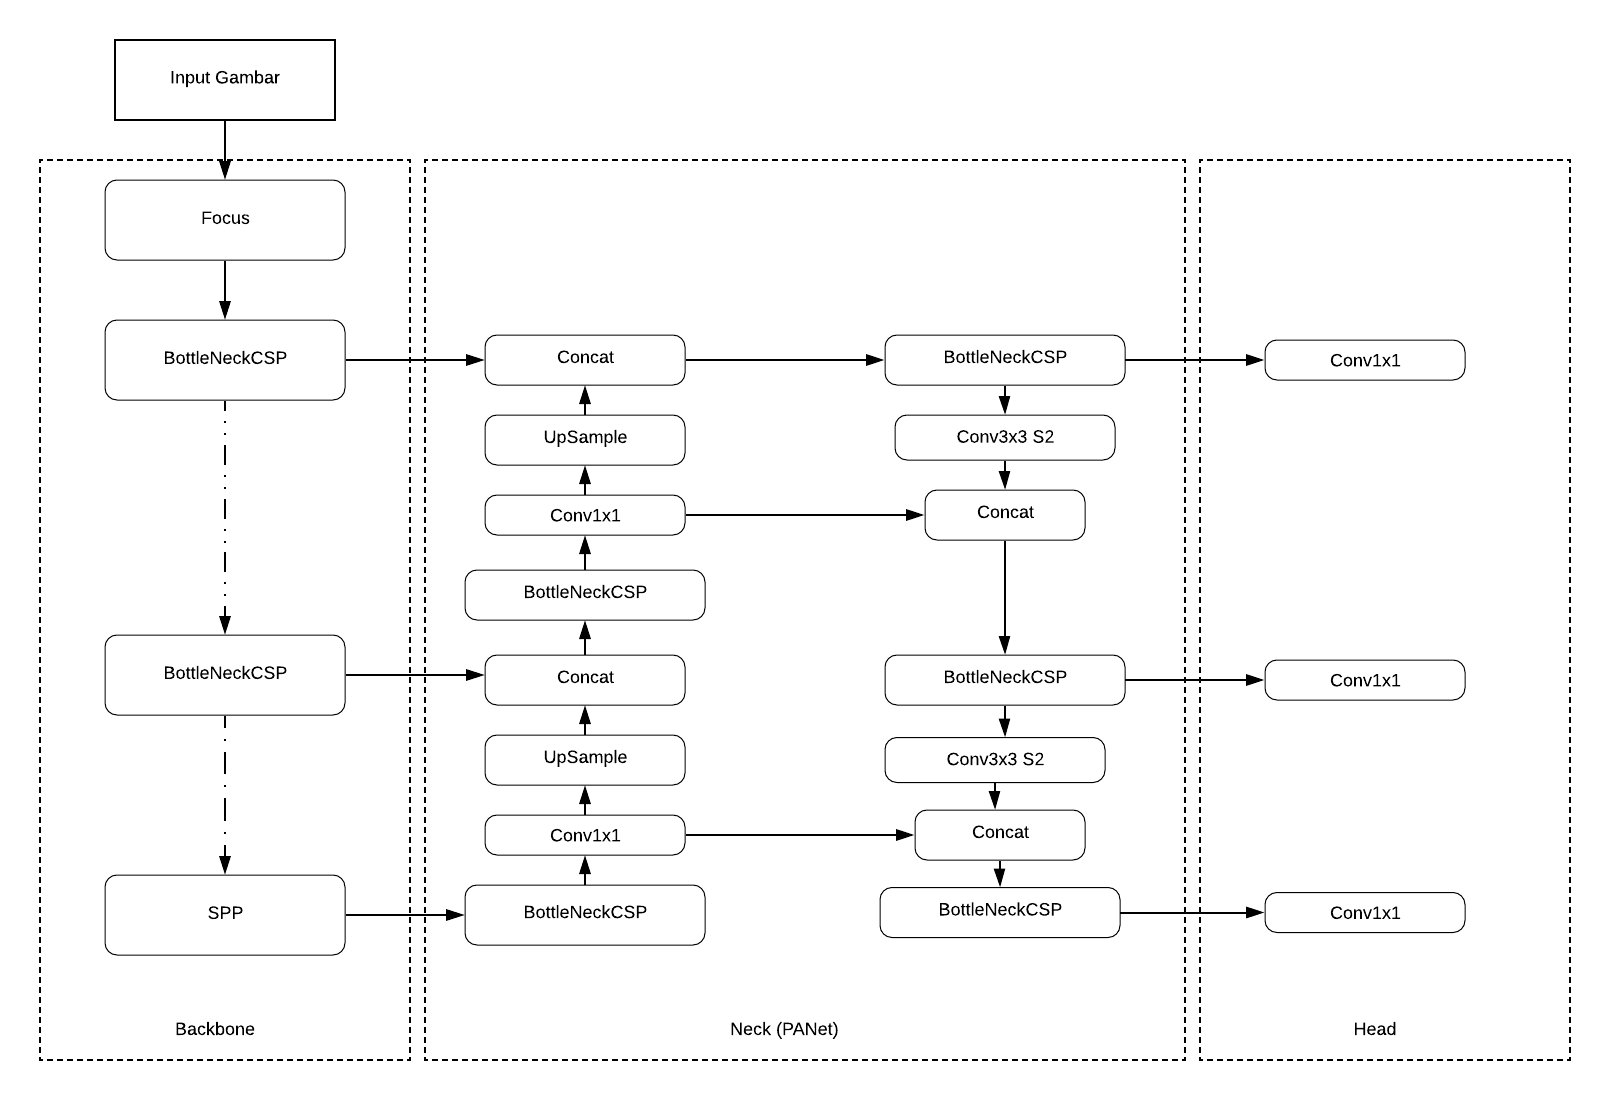
\includegraphics[scale=0.5]{gambar/yolov5 structure.png}
    \caption{Struktur Jaringan YOLOv5}
    \label{fig:yolov5network}  
\end{figure}

\par YOLOv5 merupakan versi pembaruan dari YOLO yang dicetuskan pada tahun 2020 oleh Glenn Jocher \cite{glenn_jocher_yolov5}. Berdasarkan dari \emph{repository} Github untuk YOLOv5 oleh Glenn Jocher, struktur jaringan dari YOLOv5 dibagi menjadi 3 bagian utama yaitu modul \emph{Backbone}, \emph{Neck}, dan \emph{Head}.
Seperti yang dapat dilihat di Gambar \ref{fig:yolov5network} Struktur jaringan dari YOLOv5 ini dimulai dari modul \emph{Backbone} dimana dilewati pertama oleh input gambar untuk mengekstrak fitur - fitur dari gambar yang strukturnya berbasis dari struktur \emph{Focus}, \emph{Bottleneck CSP (Cross Stage Partinal Networks)}, dan \emph{Spatial Pyramid Pooling (SPP)}.
Hasil ekstraksi fitur dari \emph{Backbone} lalu digunakan untuk menghasilkan \emph{feature pyramid} di modul \emph{Neck} yang merupakan struktur yang berbasis dari PANet (\emph{Path Aggregation Network}).
Lalu terakhir di Modul \emph{Head} dilakukan penampilan \emph{bounding box} yang meliputi beberapa informasi yaitu : kelas, koordinat, dan \emph{confidence score}.

